\chapter{Introduction}
\label{chapter:introduction}
Knowledge work has become increasingly distributed in recent years \autocite{herbsleb2001global}. This trend is caused by globalization, access to talent, cheaper labor,  and the increasing popularity of working from home \autocite{herbsleb2007global, ecoWorkingFromHome2021}. Reasons for this growing popularity include a more flexible schedule, increased work productivity, and spending less time and money on commuting \autocite{flores2019understanding, mulki2009set}. Additionally, the increased flexibility and autonomy allows employees to manage their family responsibilities better, leading to higher job satisfaction and employee retention \autocite{mulki2009set, gajendran2007good, madsen2011benefits}.

However, working remotely also brings challenges, namely that coordination and collaboration become much more difficult \autocite{herbsleb2007global}. One reason for this challenge is reduced team awareness, which is the understanding who is working on what, what they will do next, and how their actions might affect others \autocite{dourish1992awareness, herbsleb2007global, gutwin2004group}. %Workplace awareness defines awareness that results from the real-time combination of elements that workers keep in mind when collaborating \autocite{gutwin1996workspace}. Such elements can be people, what they are working on, what are are planning on working on next, which objects they are using, and more \autocite{gutwin1996workspace}.
This is because much of the implicit information (who is around, who can be disturbed, or who is currently working on what file) is no longer available \autocite{gutwin2004importance}. Consequently, a large body of research has focused on improving these coordination and collaboration challenges by increasing awareness amongst team members. The most prevalent approaches are work-related awareness tools (e.g., \autocite{biehl2007fastdash, jakobsen2009wipdash, cheng2003jazzing, deline2005easing}). These tools aim to improve collaboration efficiency by visualizing file navigation history, improving the understanding of other users' thought processes, or offering chat functionality where work-related conversations can be had, organized, and saved for later reference. 

However, previous work by \citeauthor{gutwin2004group} suggested that software developers can find all the information they need for their work even without such advanced awareness approaches \autocite{gutwin2004group}. Further, advances in commercial collaboration tools seem to develop rapidly (e.g., Google Workspace, JetBrains Space, GitHub, Microsoft Teams). For those reasons, our research focuses on more social challenges resulting from remote work, such as the scarcity of informal communication.

Due to the reduced awareness in remotely working teams, spontaneous, and often informal, communication is more difficult to initiate, and thus less prevalent in remote work \autocite{kraut1988patterns, sengupta2006research, herbsleb2007global, hinds2005understanding}. However, this is not desirable, because spontaneous or serendipitous communication, such as \enquote{corridor or watercooler talk}, accounts for about 85\% of all communication \autocite{kraut1990informal}, and can help news spread faster among teams \autocite{herbsleb2000distance} or reduce some of the coordination problems \autocite{herbsleb1999architectures} mentioned above by gathering important background information that enables more effective teamwork \autocite{lanubile2007collaboration, herbsleb2001global}. 
%Besides less frequently engaging in spontaneous, informal communication, planned communication can suffer due to technical issues with video conferencing (e.g., low bandwidth), reducing remote team productivity \autocite{sengupta2006research}. 

The lack of such social interactions can lead to other interpersonal problems, such as difficulties in building trust, maintaining working relationships, or leading to feeling disconnected from the team \autocite{comella2020revisiting, olson2006bridging}. In extreme cases, a lack of social and emotional interactions can lead to workplace isolation \autocite{marshall2007workplace, gorlick2020productivity, mulki2009set}. This is critical since feeling disconnected from colleagues has been shown to decrease engagement in productive tasks \autocite{lostFocus2020}, while strong team cohesion has been shown to positively impact team effectiveness and productivity of a team \autocite{carlson2017virtual}. Research has thus also looked into ways of encouraging more social, spontaneous interactions within remotely working teams. One approach is virtual offices, which use virtual representations of an office in which users can navigate and interact with others and have been developed both in research (e.g., \autocite{ lou2012presencescape}) and commercially (e.g., Branch\footnote{\url{https://branch.gg}}, Reslash\footnote{\url{https://reslash.co}}, Wonder\footnote{\url{https://wonder.me}}, or Gather\footnote{\url{https://gather.town}}). While \textcite{lou2012presencescape} noted an increase in informal communication through the use of their virtual worlds approach, we believe their 3D office visualization can be intrusive and therefore less suitable for everyday use in the workplace. 

Another, less intrusive concept aimed at promoting informal communication is micro-blogging in the workplace (e.g., \autocite{ebner2008microblogging, ehrlich2010microblogging, zhang2010case, dullemond2013fixing}). Micro-blogging is an informal form of communication where users can describe their current status, progress, or thoughts in short text messages and share them with other users \autocite{java2007we, dullemond2013fixing}. WeHomer, a micro-blogging tool introduced by \textcite{dullemond2013fixing}, was the first to extend a micro-blogging approach with mood sharing. Their motivation for sharing moods came from \textcite{garcia1999emotional}, who argued that being aware of the emotional state of your colleagues and acting accordingly leads to better collaborative work results.  Furthermore, the richness of communication is drastically reduced because written text, which is often used among knowledge workers, has only limited ability to convey emotional data \autocite{hook2008interactional}. By developing and studying WeHomer, \textcite{dullemond2013fixing} found an increase in team-connectedness and easy access to otherwise hard to obtain information. However, we note some limitations of their approach, namely that sharing moods was impossible without a status message, making it impossible to measure an isolated effect of sharing moods. In addition, the representation used for the moods was relatively inconspicuous by using text (e.g., \enquote{:-)}), leading us to believe that the effect of sharing moods was not very pronounced. Last but not least, responding to shared posts is only possible via commenting, which is visible to everyone else and therefore may not be ideal for more personal comments. Their findings and the fact that the COVID-19 pandemic has led to alarming numbers in employee well-being and mental health - 65.9\% of people report an increase in stress, and 44.4\% report a decrease in mental health \autocite{mswellbeing} - prompted us to develop a mood-based micro-blogging approach built on the foundation of WeHomer.

In our work, we extend WeHomer by addressing the identified limitations and studying the following key concepts:

\begin{enumerate}
    \item \textit{Focus on People and Micro-Blogging} \\
    Our approach focuses on people both visually and content-wise, and enables informal communication through mood-based micro-blogging.
    \item \textit{Spontaneous Interactions} \\
    Complementing micro-blogging, we believe that various opportunities for spontaneous interactions should be offered.
    \item \textit{Unobtrusive Design} \\ 
    Our approach focuses on moods by emphasizing them in a novel, unobtrusive user interface.
\end{enumerate}

Following these concepts, our goal is to increase social awareness and strengthen the sense of belonging. This work aims to implement those concepts in a research prototype and evaluate their potential in a small preliminary evaluation. To do this, we investigate whether there is a general need for mood sharing in the workplace (RQ1), what users share with their team (RQ2), how users use our tool (RQ3), and what the broader implications of our approach are (RQ4). Thus, the research questions we sought to answer are:

\bigskip\noindent\textit{Information Sharing}

\smallskip\noindent\textit{RQ1}: Is there a need for sharing moods/states with team members, and what are the reasons?

\smallskip\noindent\textit{RQ2}: What are knowledge workers willing to share with their team?

\medskip\noindent\textit{Tool Usage and Workflows}

\smallskip\noindent\textit{RQ3}: How do knowledge workers use and interact with a mood-based micro-blogging approach? How do they integrate it into existing workflows?

\medskip\noindent\textit{Impacts of AmbientTeams}

\smallskip\noindent\textit{RQ4}: What are the effects of  a mood-based micro-blogging approach?

\setlength{\leftskip}{0.5cm}
\smallskip\noindent\textit{RQ4.1}: Do mood and state sharing increase the awareness between team members, and how? What do they learn from each other?

\smallskip\noindent\textit{RQ4.2}: Does sharing moods and status messages affect the sharing user?

\smallskip\noindent\textit{RQ4.3}: Does AmbientTeams reduce the feeling of isolation in remote knowledge work teams?

% \smallskip\noindent\textit{RQ3.2}: Does it make users feel better to share information with their team?
% \smallskip\noindent\textit{RQ3.3}: Does it stress/relax users to see more about their team?

\setlength{\leftskip}{0pt}

\bigskip\noindent Following the concepts introduced above, we developed AmbientTeams, a desktop application that allows knowledge workers to add their most important team members and visualize them in a glanceable, transparent, and always-on-top window (see \autoref{fig:at_ambient_intro}). It differs from existing micro-blogging solutions in that it is more person- and mood-centric, and uses a novel approach to the user interface. Further, the content of textual information is de-emphasized as it is meant to complement the shared moods. These moods are visualized in mood-adapted avatars, which are the center of AmbientTeams. While \textcite{dullemond2013fixing} provides the ability to respond to shared posts with comments, AmbientTeams provides response options such as direct messaging and video conferencing to allow for spontaneous interactions. 

\begin{figure}[h]
    \centering
    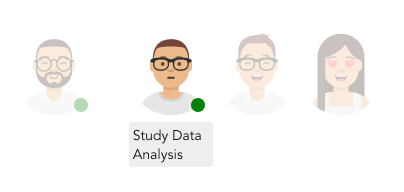
\includegraphics[width=.5\linewidth]{./images/AT_ambient_intro.png}
    \caption{AmbientTeams: Screenshot of the Glanceable, Always-on-Top Window}
    \label{fig:at_ambient_intro}
\end{figure}

% Somewhat concerning to us is the seemingly little effort to improve the situation for remote workers suffering from the perception of workplace isolation, a feeling that is referred to as 

% Consequently, there is a decrease in communication frequency when physical distance between co-workers is increased {\autocite{herbsleb2003empirical} because much of the information normally present in a co-located setting is no longer available (e.g., whether a co-worker is in an available and an interruptable state (\autocite{})). 

% The current COVID-19 pandemic makes research in the field of remote work even more important because the majority of managers expect to have more flexible work from home policies post-pandemic, and employees would like to continue working from home at least partially \autocite{msworkindexconnection}, making the topic very much relevant also after the pandemic.

% While working from home has numerous benefits, it also comes with a range of challenges. On the benefits side, employers can realize savings in real estate costs, and the employee can benefit from more flexible work hours and spending less time and money commuting \autocite{mulki2009set}. However, shared challenges from working from home are that communication is reduced \autocite{kraut1988patterns} and suffers in quality \autocite{mulki2009set}. More specifically, informal communication drastically reduces when working from home \autocite{hinds2005understanding}. This reduction of informal communication can lead to difficulties building trust, maintaining work relationships, or not feeling attached to the team \autocite{comella2020revisiting, olson2006bridging}. Another consequence of remote work is the feeling of workplace isolation \autocite{mulki2009set, marshall2007workplace}. The feeling of isolation leads to not knowing whom to turn to in case of a problem or not feeling part of the company and is said to be caused by missing support from co-workers and opportunities for social and emotional interactions in a team \autocite{marshall2007workplace}. The pandemic further reinforces this influence leading to almost 60\% feeling less connected to their co-workers compared to before the pandemic \autocite{msworkindexconnection}. Since strong team cohesion has been shown to have a positive impact on the team's effectiveness and productivity \autocite{carlson2017virtual}, and the feeling of being disconnected from colleagues have been shown to impede engaging in productive tasks \autocite{lostFocus2020}, the connectedness with the team is of particular interest to us.

% A lack of awareness causes the challenges of working remotely: less information about co-workers is exchanged, e.g., no or fewer cues are available to identify team members' interruptibility or emotional states. This missing information makes it a lot harder to find opportune moments to initiate a conversation because it is often unknown whether a person might be in a deep focus state or whether a person might be more than happy to chat. Informal communication is further challenged because serendipity is missing when working remotely because people no longer randomly bump into each other at the water cooler or the coffee machine. Therefore, improving awareness in the workplace is the foundation of our approach.

% While there are several prior approaches to improve awareness within teams by showing the current coding tasks and work items that others are working on \autocite{biehl2007fastdash, jakobsen2009wipdash}, they do not focus on the person behind that work item. They thus do not put teams into the center of attention. To make this point stronger, recent research shows concerning numbers in regards to workers' well-being and mental health, stating that the pandemic has led to an increase in stress for 65.9\% of people and 44.4\% reported a decrease in mental health \autocite{qualtricksmental}. Therefore, our concept, AmbientTeams, follows a different approach by \enquote{putting people first}. It includes an ambient always-on-top overview of the core team members and their moods, status messages, and other states. In addition to such a micro-blogging approach, where team members can share information about their moods (and potential context), we aim to study further possibilities to foster and motivate serendipitous, informal exchanges with the team.

% In the next chapter, existing approaches and their underlying concepts are discussed before introducing our approach and its differences. The resulting prototype is then introduced in \autoref{chapter:prototype} and analyzed in the scope of a preliminary evaluation in \autoref{chapter:preliminary_evaluation}.


\bigskip\noindent To answer the research questions, we conducted a preliminary evaluation with five knowledge workers who used AmbientTeams for one week \textit{in-situ}. The participants confirmed the importance of staying aware of their co-workers' moods. Consequently, the mood-sharing functionality was the most popular feature among participants, primarily used without an attached status message. Regarding the broader effects of AmbientTeams, we found that it helped knowledge workers to 1) be more aware of each other's moods and availability status, 2) get to know each other better, 3) foster communication outside of AmbientTeams, and 4) spur self-reflection on one's moods. To summarize, the main contributions of this work include:

\begin{enumerate}
    \item Development of a mood-based micro-blogging approach with spontaneous interaction capabilities.
    \item Preliminary evaluation resulting in insights on awareness increase and micro-blogging behavior in remote teams and design considerations for such tools.
\end{enumerate}

%\begin{enumerate}
 %   \item Insights into mood and status sharing behaviors within knowledge work teams and the impact such sharing can have on personal relationships, workplace isolation, or collaboration
  %  \item Successful development of a glanceable, always-on-top status sharing window, and initial insights into the usability of such an approach
   % \item Provision and initial application of a study design that can be used for a broader study, and resulting suggestions for future features
%\end{enumerate}

The thesis starts with an overview of related work in \autoref{chapter:related_work} and continues with a discussion of the approach and its key concepts in \autoref{chapter:approach}. Subsequently, our research prototype and all its features are presented in \autoref{chapter:prototype}. The study design for the preliminary evaluation conducted can be found in \autoref{chapter:preliminary_evaluation} and the results in \autoref{chapter:results}. Last but not least, our findings are discussed and possible future directions of our approach are outlined in \autoref{chapter:discussion}.